\documentclass{beamer}
\usepackage[utf8]{inputenc}
\usetheme{Berkeley}
\setbeamercolor*{frametitle}{parent=palette primary}
\usepackage{graphicx}
\usepackage[T1]{fontenc}
\usepackage[utf8]{inputenc}
\usepackage{lmodern}
\usepackage{mwe}
\usepackage{babel}
 \usecolortheme[RGB={115,90,110}]{structure}
\title{Projet Sokoban}
\author{Guillaume \and Ronan \and Alexis \and Aboubacar}
\institute{Université de Caen Normandie \\ Conception logiciel}

\begin{document}

\begin{frame}
\titlepage
\end{frame}


\begin{frame}{Sommaire}
\tableofcontents
\end{frame}
\frametitle{Introduction}
\section{Introduction} 
\begin{frame}

\begin{figure}
        \centering
        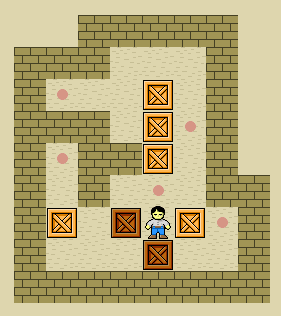
\includegraphics[scale=0.3]{../picture/WIKIPEDIA.png}
\end{figure}
\begin{figure}
        \centering
        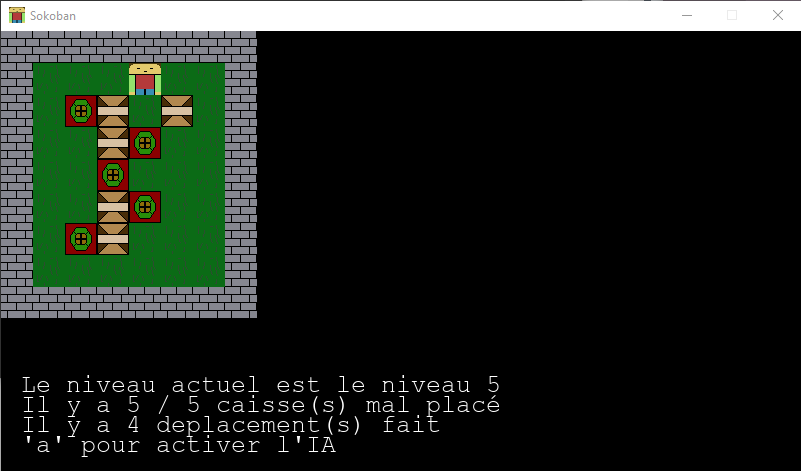
\includegraphics[scale=0.3]{../picture/monjeu.png}
\end{figure}
\end{frame}

\section{Objectif du projet}
\begin{frame}
\begin{block}{3 Grand axes du jeu :}
- Partie de séléction du niveau \\ 
- Partie jeu  \\
- Partie victoire \\
\end{block}
\begin{block}{2 Grand axes de l'IA :}
- Algorithme A* \\ 
- Noeuds \\
\end{block}
\end{frame}


\begin{frame}
\section{Fonctionalités implémentées}
\frametitle{Fonctionalités implémentées}
\begin{block}{Les fonctionalités}
Mouvement sur 2 axes \\
Déplacement de boîtes \\
Choix du niveau \\
Solution donner par l'IA
\end{block}
\begin{block}{Organisations du projet}
Guillaume: codé le jeu \\ 
Alexis: créé les maps \\
Aboubacar: crée les maps  \\
Ronan: créé les maps, Et a fait tout l'IA
\end{block}
\end{frame}

\section{Element technique}
\begin{frame}{Element technique}

\begin{block}{Fonction move :} 
- Teste les possibilités \\
- Déplace les caisses ou non \\
- Actualise la matrice en prennant en compte les mouvement \\ s'il y en a \\
\end{block}
\begin{block}{Fonction chose level:} 
- Analyse la valeur entrée ( 0 = aléatoire) \\
- Ouvre le fichier XSB  \\
- Crée les coordonnées du personnage, caisse, mur ect... 
\end{block}
\end{frame}

\section{Architecture du projet}
\begin{frame}{Architecture du projet}
\begin{figure}
        \centering
        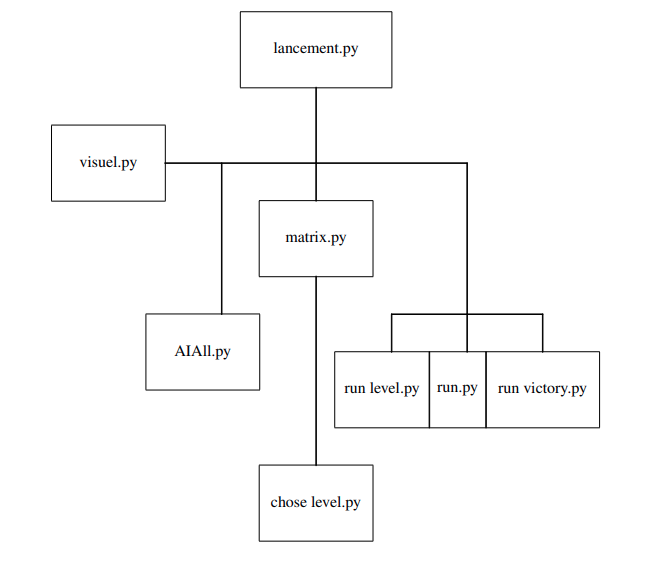
\includegraphics[scale=0.5]{../picture/archi.png}
\end{figure}

\end{frame}

\section{Expérimentation}
\begin{frame}{Expérimentation}
\textbf{Mise en fonctionnement:} \\
- La phase de selection de niveau. \\
- La phase d'éxécution du niveau.\\
- Et la phase de relancement ou non du jeu. \\
\end{frame}


\section{Conclusion}
\subsection{Récapitulatif}
\begin{frame}{Conclusion/Récapitulatif}
On a réussi a accomplire les objectifs que l'on s'est fixer, les deux éléments important que l'on voulait finir fonctionnent. \\
L'IA  peut être fortement améliorer car celle  ci peut être très longue.

\end{frame}

\subsection{Amélioration}
\begin{frame}{Conclusion/Amélioration}

\textbf{Les améliorations de notre sokoban pourrait-être:}\\
 - Animation déplacement \\
 - Sound design \\
 - Faire que l'utilisateur puissent créer ces propres niveaux \\
 - Crée une interface graphique \\
 - Caisse change de couleur si bien placé
\end{frame}
\end{document}
